%%%%%%%%%%%%%%%%%%%%%%%%%%%%%%%%%%%%%%%%%%
%
% Cosecivi 2017
% http://gaia.fdi.ucm.es/sites/cosecivi17
% 12 pages max
%
%%%%%%%%%%%%%%%%%%%%%%%%%%%%%%%%%%%%%%%%%%

\documentclass{llncs}

\usepackage{float}
\usepackage[english]{babel}
\usepackage[utf8]{inputenc}
\usepackage{epsfig}
\usepackage{graphicx}
\usepackage{subcaption}
\captionsetup{compatibility=false}
\usepackage{color}
\usepackage{amsfonts}
\usepackage{amsmath}
%\usepackage{mathabx}
\usepackage{hyperref}

%\usepackage{hyperref}
%\usepackage{subfigure}
%\usepackage[colorinlistoftodos, textwidth=3.2cm, shadow]{todonotes}

%\usepackage{algorithm}
%\usepackage{fixltx2e}
%\usepackage{algpseudocode}

%\usepackage{multirow}

% To use Call inside another Call (algorithms)
%\MakeRobust{\Call}

\graphicspath{{images/}}

\newcommand{\pacman}{Ms. Pac-Man vs. Ghosts }
\newcommand\tab[1][1cm]{\hspace*{#1}}
\newcommand{\paco}{Pac-Man }

%%%%%%%%%%%%%%%%%%%%%%%%%%%%%%%%%%%%%%%%%%
%
% Title
%
%%%%%%%%%%%%%%%%%%%%%%%%%%%%%%%%%%%%%%%%%%
\title{Title\thanks{Supported by Spanish Ministry of Economy and Competitiveness under grants TIN2014-55006-R and TIN2014-57028-R}
}

\author{{\color{red} los que faltan}, José Miguel Tajuelo Garrigós, Jorge Vieira Luna, Carlos Cervigon Rückauer, Antonio A. S\'{a}nchez-Ruiz}

\institute{
	Dep. Ingenier\'{\i}a del Software e Inteligencia Artificial \\
	Universidad Complutense de Madrid (Spain) \\
	\email{{\color{red} los que faltan}, jtajuelo@ucm.es, jovieira@ucm.es, {\color{red} correo de carlos}, antsanch@ucm.es}
}

\begin{document}

\maketitle

%%%%%%%%%%%%%%%%%%%%%%%%%%%%%%%%%%%%%%%%%%
%
% Abstract
%
%%%%%%%%%%%%%%%%%%%%%%%%%%%%%%%%%%%%%%%%%%
\begin{abstract}
Bla bla bla ... 
Dejar para el final

\keywords{keyword1, keyword2, ...}
\end{abstract}

%%%%%%%%%%%%%%%%%%%%%%%%%%%%%%%%%%%%%%%%%%
%
\section{Introduction}
\label{sec:intro}
%
%%%%%%%%%%%%%%%%%%%%%%%%%%%%%%%%%%%%%%%%%%

Dejar para el final

{\color{red}CARLOS: Antes del apartado 2 ¿no sería bueno meter un apartado Previous Work con referencias a todo lo que se ha hecho en Pacman con Gramáticas evolutivas y programación genética?. Veo que está en el apartado 5 Related Work}

%%%%%%%%%%%%%%%%%%%%%%%%%%%%%%%%%%%%%%%%%%
%
\section{\pacman AI}
\label{sec:pacmanai}
%
%%%%%%%%%%%%%%%%%%%%%%%%%%%%%%%%%%%%%%%%%%


\begin{figure}[H]
	\centering
	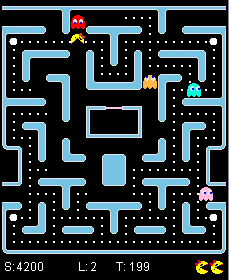
\includegraphics[width=8cm]{images/PacMan_ss.png}
\end{figure}


\begin{itemize}

\item The game
\\

In the version of the game we use {\color{red}(referencia a su git)} there is a set of four pregenerated toroidal 2D labyrinths, in which the ghosts and \paco move. The ghosts always start in the "Lair", a rectangle in the middle of the map in which \paco cannot enter. \paco starts in the bottom of the map.

Each labyrinth is composed of corridors and junctions filled with a lot of pills and four powerpills. Both give points to \paco as he walks over them, and powerpills make him able to eat the ghosts for a short period of time, while also slowing them. Eating ghosts will give \paco points, earning some extra ones if he eats various ghosts in a row during the same powerpill buff duration.

\paco will try to eat all the pills and powerpills to advance levels, while avoiding the ghosts, which will try to hunt him, making him lose a live when they walk over him. A level is completed when there are no pills or powerpills left, and there are an infinite number of levels, repeating the same set of 4 labyrinths consecutively.

\paco will strive to eat all the pills and powerpills in the map to advance levels, while trying to get as much points as possible eating any ghosts he can, since each 10.000 points achieved he gets an extra life.

The game ends either when \paco loses his three lives or after 24.000 turns, considering a turn passes every time both \paco and the ghosts make a movement.
\\
\\

\item Bot implementation architecture
\\

Both the ghosts and \paco use controllers to determine which movement is the best to make every turn. These controllers are the ones that must be implemented to participate in the competitions, which can be done using any technique available.

Every turn the game provides the controllers with its current state, so that the controller can seek relevant information it needs to choose a movement. Such information includes the pre-calculated distance from a point of the map to another (useful to check distances between \paco and the ghosts), which is the movement that puts you further away from any other position (useful to run away from the ghosts), which movements are possible given a position, testing if a position is a junction or not, etc. 

We've greatly increased the information to obtain by combining those given functions, like getting a movement towards the closest junction, the closest edible ghost, or the closest powerpill.

{\color{red}optar por "nosotros no hemos tenido en cuenta esta estructura para crear una interfaz que permita investigar diferentes técnicas de evolución gramátical combinadas" o pasar todo a formato concurso. Jorge:Veo mas viable lo primero. Josemi: +1. ANTONIO: como que no habéis tenido en cuenta esta estructura?}
\\
\\

\item Previous competitions
\\

\paco has been used in many bot implementing competitions, of which the most important are:

\begin{itemize}
\setlength{\itemindent}{-.3cm}
\item "Ms Pac-Man Competition"{\color{red} link a http://dces.essex.ac.uk/staff/sml/pacman/PacManContest.html}

This competition took place six times between 2007 and 2011. It used a different architecture to ours in which the participants had to capture the screen of the game to obtain game status information. 
\item "Ms. Pac-Man Vs. Ghost Team Competition"{\color{red} link a http://www.pacmanvghosts.co.uk/}

Currently active, this competition was held in CIG 2016{\color{red} link a http://www.pacmanvghosts.co.uk/files/ms-pac-man.pdf} and is to be held again in 2017. It uses our same base architecture, although in their implementation the visibility of the agents is limited by "Partial Observability", in which both \paco and the ghosts can only obtain information of the game that is in their line of sight, this is, the corridor they are in or, if they are in a junction, the corridors that cross that junction.
\end{itemize}

 


\end{itemize}


%%%%%%%%%%%%%%%%%%%%%%%%%%%%%%%%%%%%%%%%%%
%
\section{A bot based on grammatical evolution}
\label{sec:sec1}
%
%%%%%%%%%%%%%%%%%%%%%%%%%%%%%%%%%%%%%%%%%%

\begin{itemize}
\item Idea general
\item Parámetros que definen el estado de juego
\item Acciones
\item Gramática
\item Frameworks utilizados
\item Operadores de cruce y mutación
\item Resultados (¿comparación con otros bots?, ¿estrategias aprendidas?)
\end{itemize}

{\color{red}ANTONIO: no hace falta crear subsecciones para todo}

\subsection{General idea}

{\color{red}ANTONIO: la idea general es usar Grammatical Evolution para construir programas que juegan automáticamente. En particular, vamos a generar programas que juegan de manera puramente reactiva, es decir, que toman decisiones basadas en el estado actual del juego pero no tienen en cuenta las decisiones tomadas previamente. De este modo, esperamos obtener programas sencillos pero que no son capaces de codificar explícitamente estrategias complejas consistentes en secuencias de acciones.}

Since the beginning we decided to take a Grammatical Evolution approach. This means evolving several solutions or expressions, which belong to the language generated by a user defined context-free grammar, more precisely a Backus-Naur Form denoted grammar. 

By using Grammatical evolution we were able to reduce and refine the search space the evolutionary algorithm will explore, deciding to generate only Reactive Artificial Intelligence based bots. This type of Artificial Intelligence first evaluates the world and then executes and actions, following in our case condition-action rules defined by the grammar

{\color{red}ANTONIO: ejemplo de un programa interesante y explicarlo. Decir que, en el fondo, estamos construyendo árboles de decisión donde los nodos intermedios toman decisiones en función del estado de la partida, y las hojas son las acciones concretas a ejecutar por el bot.}

\subsection{Frameworks}

{\color{red}ANTONIO: aquí no pega, contar más adelante}

We use the \paco implementation described in section 2 as our starting point, integrated with JECO (\textit{Java Evolutionary COmputation library}) {\color{red} link a https://github.com/jlrisco/jeco}. JECO is a framework which supports different evolutionary computation techniques, including what we wanted to try in \paco: Simple and multi-objective grammatical evolution.


\subsection{Actions and functions}

{\color{red}ANTONIO: Esto enlaza muy bien con el ejemplo de programa. Explicar las acciones y las funciones usando itemize en lugar de tablas (el texto queda demasiado pequeño). Luego habáis de 2 gramáticas pero no queda claro que acciones aparecen en cada una.}

In order to allow our bot to interact with the game, we had to create two categories of methods:

\subsubsection{Actions}
Methods which result in a move for the bot to execute.
\subsubsection{Functions}
Methods which check a boolean condition or obtain a numeric value of the game state at a moment, allowing the bot to get information of the current state of the game.

\begin{table}[]
\centering
\resizebox{\textwidth}{!}{%
\begin{tabular}{|l|l|}
\hline
Action & Description \\ \hline
getDirectionTowardsClosestPill & obtains a move towards the closest pill using A* search \\ \hline
getDirectionAwayFromClosestNonEdibleGhost & obtains a move away from the closest non edible ghost using A* search \\ \hline
getDirectionTowardsClosestEdibleGhost & obtains a move towards the closest edible ghost using A* search \\ \hline
getDirectionTowardsClosestPowerPill & obtains a move towards the closest power pill using A* search  \\ \hline
\end{tabular}%
}
\caption{Actions used}
\label{my-label}
\end{table}

\begin{table}[]
\centering
\resizebox{\textwidth}{!}{%
\begin{tabular}{|l|l|}
\hline
Funcion & Description \\ \hline
getDistanceToClosestNonEdibleGhost & obtains distance to closest non edible ghost using A* search \\ \hline
getDistanceToClosestNonEdibleGhost(directional) & obtains distance to closest non edible ghost using A* search and following a direction \\ \hline
getDistanceToClosestEdibleGhost & obtains distance to closest edible ghost using A* search \\ \hline
getDistanceToClosestEdibleGhost(directional) & obtains distance to closest edible ghost using A* search and following a direction \\ \hline
getNumberOfActivePowerPills & obtains the number of active power pills \\ \hline
getDistToClosestPill & obtains the distance to the closest power pill \\ \hline
getDistToClosestPill(directional) & obtains the distance to the closest power pill following a direction \\ \hline
getJunction & checks if \paco is currently at a junction \\ \hline
\end{tabular}%
}
\caption{Functions used}
\label{my-label}
\end{table}

\subsection{Grammars}

{\color{red}ANTONIO: poned las gramáticas en BNF y explicadlas por encima.}

Because the usage of grammars, we decided to design two grammars, both including said condition-action rules, like if(cond){action} and if(cond){action}else{action} ({\color{red} bloque de codigo})

However, one of the grammar only includes low to medium level actions and functions, and the other including high-level actions and functions, being the second a result of the inclusion of expert knowledge({\color{red} mencionar sistemas expertos?!}).

Finally, both grammars include discrete numbers, much more efficient than ranges, and numeric operators (==, !=, >, >=, <=, <) ({\color{red} bloque de codigo}) for the numeric data treatment, as well as boolean operators (!, and, or) ({\color{red} bloque de codigo}) for the boolean data treatment.

\subsection{Operators}
The usage of the Grammatical Evolution algorithm requires using crossover and mutation operators. We have implemented and tested several operators, including: ({\color{red} lista})
After said tests comparing selection, elite, crossover and mutation operators as well as their hyper-parameters, we obtained the best results using: Tournament selection with elite, LHS crossover and or combinatorial or swap mutation ({\color{red} completar})

{\color{red}ANTONIO: cual es la función de fitness? la que contáis en el apartado siguiente? pues traedla aquí}

\subsection{Results}

{\color{red}ANTONIO: antes de contar las estrategias mostrad los resultados: gráfica de fitness vs. generaciones, tabla comparativa con otros bots (aleatorio, legacy, ...) poniendo los metaparámetros usados (prob mutación, elite, etc), hablar de la longitud de los programas generados. Todo esto para cada gramática. }

After analysing the results after each execution we discovered several facts. 

First of all, most executions using the medium-level grammar were able to find a bug on the ghost starter controllers, exploiting it and being able to complete endless levels.

After that discovery we decided to use a significantly harder ghost bots ("Legacy 2: The Reckoning" ghost controller). However, the new bots generated using the medium-level grammar tend to generate bots which manage to get stuck next to power pills (stopping themselves), wait for the ghosts to be close and proceeding to eat first the power pill and then the ghosts, now edible. This hunter behaviour allows \paco bots to achieve notable scores, but happens to be a local minimum.

Finally, the bots generated by the high-level grammar share almost almost always the same code, and achieve even higher scores, eating pills conservatively by avoiding ghosts.

% he escrito un poco y resulta que tú tienes lo mismo, te lo dejo aquí por si te sirve
%\paragraph{Camper}
%\paco abuses ghost eating multiplier by waiting around a joint until enough ghosts appear. Then eats a power pill and begins hunting close edible ghosts, reaching a score of $11000$ points very quickly. This is the result of optimize vanilla \pacman score \ref{vanilla_pacman_score}.

({\color{red} bloque de codigo})

%%%%%%%%%%%%%%%%%%%%%%%%%%%%%%%%%%%%%%%%%%
%
\section{Multi-objective optimization}
\label{sec:sec3}
%
%%%%%%%%%%%%%%%%%%%%%%%%%%%%%%%%%%%%%%%%%%

\begin{itemize}
\item En qué consiste el multi-objetivo
\item por qué es interesante considerar varios objetivos en el juego
\item Experimentos y resultados  ¿estrategias aprendidas?)
\end{itemize}

\subsection{Definition}

{\color{red}ANTONIO: referencia al artículo donde se define este tipo de optimización. No entiendo esa fórmula (que es F, G y H), poned sólo lo que sea necestio para explicar en qué consiste.}

Multi-objective optimization arises when a single objective with several constraints may not adequately represent the problem being faced. It can be formulated as
\begin{equation}
\begin{aligned}
& \underset{x}{\text{min}}
& & F(x) = [f_1(x), f_2(x), \cdots, f_k(x)] \\
& \text{s.t.} & &  G(x) = [g_1(x), g_2(x), \cdots, g_m(x)] \leq 0 \\
& & &  H(x) = [h_1(x), h_2(x), \cdots, h_m(x)] = 0 \\
\end{aligned}
\end{equation}

If some objective function is to be maximized, it is equivalent to minimize its negative.

Note that because $F(x)$ is a vector, if two or more of the components of $F(x)$ are conflicting, there is no unique solution to this problem. Instead, the concept of non-domination, also non-inferiority called Pareto optimality \cite{Censor:78}, must be used to characterize the objectives. A non-dominated solution is one in which it is not possible to move feasibly from it to increase an objective without decreasing at least one of the others.

{\color{red}CARLOS: creo que habría que explicar bien lo de los óptimos de Pareto y las soluciones no dominadas}


% https://en.wikipedia.org/wiki/Multi-objective_optimization
% https://ocw.mit.edu/courses/engineering-systems-division/esd-77-multidisciplinary-system-design-optimization-spring-2010/lecture-notes/MITESD_77S10_lec14.pdf

\subsection{Why to apply it}

{\color{red}ANTONIO: esto no va en el apartado 3?}

Our initial (\textit{fitness}) function to optimize was
\begin{equation} % label: naivefitness
f = 10000 - score
% caption: Naive fitness
\end{equation}
(note that we are minimizing).

Score points, as originally defined in the source code for \pacman competition, are gained applying the following criteria:
\begin{itemize}
\label{vanilla_pacman_score}
\item Eat pill: $10$ points.
\item Eat power pill: $50$ points.
\item Eat ghost: $200$ points ($200x$ when eating in a row).
\end{itemize}

This, when using a single objective function that maximizes score, inevitably leads to bots that keep moving around a power pill until one or more ghosts approach. Then \paco eats the power pill and proceed to eat as many ghosts as possible, making good profit out of it.

{\color{red}ANTONIO: a partir de aquí sí}

This strategy only works when there are still power pills available. With no power pills left, \paco keeps rambling until a ghost eats it and the game is over. So it is clear that we need to counterbalance ghost score to pass to next level.

Instead of overcomplicating the objective function trying to fulfil several goals, we simply define several objective functions in charge of different desirable aspects of the bots.
{\color{red} necesitamos un argumento más convincente, con pruebas hechas incluso}

\begin{equation}
f_2 = 100 - \text{last level reached}
% caption: levels completed
\end{equation}

We can even define the vanilla score function without the ghost multiplier.
\begin{equation}
\begin{split}
f_3 = 100000 - & (\text{pills eaten} \times \text{pill score} \\
& + \text{power pills eaten} \times \text{power pill score} \\
& + \text{ghosts eaten} \times \text{ghost score}) \\
% caption: no ghosts multiplier
\end{split}
\end{equation}

With a combination like $F = [f_2, f_3]$ a working multi-objective function can be created.

\subsection{Exp}
{\color{red} No hay resultados porque no hay suficientes pruebas multi-objetivo, ni ideas para pruebas. Por tanto tampoco datos para graficar. Los únicos experimentos y gráficos que hay pueden verse aquí \url{https://github.com/hecoding/Pac-Man/tree/measurements}}

{\color{red}ANTONIO: comparar el multiobjetivo con los resultados del apartado anterior. Al menos se pasará más niveles, aunque consiga peor puntuación...}

\subsubsection{Learned strategies}
{\color{red}No hay estrategias conocidas exclusivamente debidas a multiobjetivo, que sepa.}

%%%%%%%%%%%%%%%%%%%%%%%%%%%%%%%%%%%%%%%%%%
%
\section{Related Work}
\label{sec:relatedWork}
%
%%%%%%%%%%%%%%%%%%%%%%%%%%%%%%%%%%%%%%%%%%

{\color{red}ANTONIO: no hay que explicar las cosas como si fuera un libro de texto, hay que referenciar los trabajos científicos más relevantes (relacionados con lo que hemos hecho) y decir cual es la aportación de cada uno y en que se diferencia lo que hemos hecho nosotros.}

{\color{red}CARLOS: Los apartados de este punto 5 no veo que tengan sentido contarlos al final. Yo los pondría entre los apartados 1 y 2, explicando en orden las diferentes técnicas: programación genética, gramáticas evolutivas, decision trees, behavior trees. ; luego pondría referencias a los trabajos que se han hecho en cada área: Ejemplo ver apartado II: http://geneura.ugr.es/cig2012/papers/paper8.pdf

...y la parte de multiobjetivo debería ir entonces al apartado 4}


\subsection{Decision Trees and Behaviour Trees}

Decision Trees are a special type of graphs commonly used in Artificial Intelligence to represent complex outputs depending on different conditions. These conditions are evaluated by the inner nodes of the tree, usually called conditional nodes, which depending on the output of the condition they hold they set which child node to process. Terminal nodes are the outputs that will be obtained from the decision tree. 
%$http://www.aihorizon.com/essays/generalai/decision_trees.htm$ 
Decisions trees are fast to process once build and can model complex decision schemes and strategies. The main drawback is the incapacity of outputting more than one action, each execution of a Decision Tree outputs a single deterministic action based on the current state of the environment variables.

Behaviours trees can be seen as a different way of representing Finite States Machines (FSM). They were developed to avoid the exponential growth of FSMs representing the AI of NPCs in video games. Their structure is similar to the one of a Decision Tree but with more types of inner nodes, like loop nodes, which enables the encode of more complex decision schemes and strategies outputting several possible actions in a single execution of the tree.
%$http://gaia.fdi.ucm.es/sites/cosecivi14/es/papers/27.pdf$
\subsection{Genetic Programming}
Genetic Programming is one of the many different branches of algorithms that exist inside Evolutionary Algorithms.
%Libro de Carlos
Genetic Programming tries to produce the best program, in a determined programming language, using an Evolutionary Algorithm approach. The programs are encoded using trees (genome)  in which each node represents a token of the chosen programming language, hence each individual of the population is a program which will be selected, crossover and mutated using different selection, crossover and mutation operators and his genome will be transformed into the final program (phenotype) and will be evaluated. This process is repeated several times and the final solution will be the individual with the program with the best score of the whole population. A problem with Genetic Programming is that the use of trees to encode the genome is very heavy in terms of memory specially when bloating occurs.  %$https://link.springer.com/book/10.2991/978-94-6239-255-7#page=190$
%$http://ieeexplore.ieee.org/abstract/document/7849864/$
%$https://link.springer.com/chapter/10.1007/978-3-319-49001-4_4$
%$https://link.springer.com/chapter/10.1007/3-540-36599-0_19$
\subsection{Grammatical Evolution}
Grammatical Evolution is similar to Genetic Programming in that both evolve programs to find the best one but the encoding of the programs (genotype) in Grammatical Evolution is different. Now, the genotype is an array of integers where each integer represents the rule of a grammar, written in Backus-Naur Form,
%http://www.garshol.priv.no/download/text/bnf.html
that will be chosen to produce the program (phenotype) when the genotype is decoded. So now the process of crossover and mutation is done with the array, increasing performance in time and memory and thanks to BNFs languages are very easy to design and change without reimplementing or modifying the algorithm code.%O'Neill, M. and Ryan, C. (2003). Grammatical Evolution. 1st ed. Boston, MA: Springer US.

With this new representation of the genotype some new crossover and mutation operators work better than the classical ones like LHS replacement crossover, which tries to do the crossover less destructive,
%Harper, R. and Blair, A. (n.d.). A Structure Preserving Crossover In Grammatical Evolution. 2005 IEEE Congress on Evolutionary Computation.
and Neutral Mutation. %DOI: 10.1007/978-3-319-11313-5_39

\subsection{Multi-Objective Optimization}
Single-objective optimization is mainly used with Grammatical Evolution because it's implementation is straight forward, the algorithm remains the same, there is no need of using special operators and the fitness functions is a direct translation of the problem to solve. This approach is usually effective but for complex problems it's difficult to optimize it with only one fitness function (e.g. one objective).

Multi-objective optimization tries to assort this problem using a Non-dominated Sorting Genetic Algorithm II (NSGAII). NSGAII uses Pareto Front %ISSN 1619-7127 or ISSN 978-3-540-72963-1 Multiobjective Problem Solving from Nature: From Concepts to Applications
for selecting the individual for crossover and mutation, ranking and choosing them in a tournament like way, choosing the one that has the overall best fitness in all the objectives. This individuals are known as Pareto's first optimal front or Rank 1 where other individuals, depending on their objectives fitness, will be in Rank 2, 3, etc. Pareto Front is an elitist reproduction strategy as it always try to choose the best elements of the population (Rank 1), making the best elements to survive. %https://eprints.soton.ac.uk/194307/1/Nasu_11.pdf

%%%%%%%%%%%%%%%%%%%%%%%%%%%%%%%%%%%%%%%%%%
%
\section{Conclusions}
\label{sec:conclusions}
%
%%%%%%%%%%%%%%%%%%%%%%%%%%%%%%%%%%%%%%%%%%


Dejar para el final

Añadir al final la URL al repositorio de GitHub
\url{https://github.com/hecoding/Pac-Man}

\bibliographystyle{splncs}
\bibliography{references}

\end{document}
